%\documentclass[a4paper, 12pt]{article} 


\documentclass[11pt,a4paper]{article}
\usepackage[hyperref]{acl2020}
\usepackage{times}
\usepackage{latexsym}
\renewcommand{\UrlFont}{\ttfamily\small}
\usepackage{todonotes}
\usepackage{csquotes} % Context sensitive quotation facilities
\MakeOuterQuote{"}
\title{Robust Parse Tree Features for Authorship Attribution}
\author{Anthony Chen \\ Hunter College \And Blake Vent\'e \\ Hunter College}
\date{14 December 2020}
\aclfinalcopy % Uncomment this line for the final submission
\usepackage{caption}
\usepackage{subcaption}
\usepackage{algpseudocode}
\usepackage{booktabs}
\usepackage{qtree}
\begin{document}
\maketitle
%-------------------------------
%	TITLE SECTION
%-------------------------------


\begin{abstract}
We extend prior work on path-based constituency parse tree features for robust authorship attribution. We reach an $F_1$ score of 72 percent using TF-IDF on unigrams up to trigrams of the extracted parse tree paths of length 1. Raw word counts bring our best $F_1$ score up to .94. Since the parse tree remains intact despite word-level obfuscation, this suggests that anonymity requires meaning-preserving tree-based transformations or more drastic measures as opposed to dictionary-based obfuscation.
\end{abstract}


\section{Introduction}

We perform authorship attribution (AA) on the Yelp academic dataset. Given an input sample, $x$, we use machine learning
determine which $y$ from our set of known authors wrote sample $x$ (a re-formulation of Closed-World Author De-anonymization \cite[2]{caliskan2015}). To do this, we extract parse tree features for use as a stylometric tool to distinguish authors. In the literature, token-independent path-based features have a history in (AA) for source code, but not natural language. This work takes intuitions from valuable features for source code and applies it to natural language. \footnote{We host our work at \url{https://github.com/rvente/NLP-Final-Project} }

\section{Prior Research}

Published in 2017, \citeauthor{sari-etal-2017-continuous} discusses $n$-gram feature representation for English language author attribution (AA). Later, the same researchers reach state of the art results when training a neural network to embed the contents of a document before performing AA. The differences in performance when effort is spent in choosing the features and hyperparameters are considerable \cite[9]{sari-etal-2018-topic}. Although the word-embedding based vectorizer in \cite{sari-etal-2017-continuous} may be useful for future research, we proceed using $n$-gram based vectorizers mentioned in those works to isolate word counts as a baseline.

\begin{figure*}
    \centering
     \begin{subfigure}{0.30\textwidth}
    \centering
\Tree [.S [.NP [.DT This ] ] [.VP [.VBZ is ] [.NP [.DT an ] [.NN orange. ] ] ] ]
         \caption{Corresponding features}
         \label{fig:tree}
     \end{subfigure}
 \begin{subfigure}{0.65\textwidth}
  \begin{tabular}{||l l ||} 
 \hline
 Feature Set & Example \\ [0.5ex] 
 \hline\hline
  POS tags & S NP VP DT VBZ NP DT NN   \\

 nested  bigrams & S↓NP S↓VP NP↓DT VP↓VBZ VP↓NP   \dots \\
 POS paths L1 & \emph{above plus} S↑ROOT NP↑S DT↑NP  \dots \\
 POS paths L2 & S↓NP↓DT \dots NP↓DT↓PAD \dots NP↑S↓VP  \dots \\

 \hline
\end{tabular}
    \centering
         \caption{L1 and L2 abbreviate length 1 and length 2. In adherance with the \citeauthor{2001.11593} we also call L1 paths "path bigrams" and L2 paths "path trigrams". }
         \label{fig:tree_table}
     \end{subfigure}
\caption{Examples for each set of path based features set. This example documents features operating on English language. But they have also been used for authorship attribution in source code. Formally, this feature representation can be viewed as an ordered tuple of length $2n+1$ where every even numbered element is an arrow token $\in$ \{↓, ↑\}, e.g.\ (S, ↓, NP) Without loss of generality, a practical implementation can represent each tuple as a single contiguous string, with spaces delimiting the tokens in the document. This is the form illustrated in the example.}
    \label{fig:parse_tree_eg}
\end{figure*}


\citeauthor{2001.11593} developed a programming language-agnostic framework for
feature extraction for authorship attribution. In general, their PbRF model state-of-the-art accuracy even when the number of samples is relatively low.



\citeauthor{caliskan2015}'s 2015 work tackles the programmer de-anonymization problem and changed the
state of the art by focusing so heavily on nesting and intermediate
representations of source code \cite[1]{caliskan2015}. The work also proposed the same
random forest ensemble classifier used in \cite{2001.11593}. The work's dataset
- Google Code Jam - was selected as a particularly difficult sub problem: all of
the code solved the same problem so the model could not rely on the "topic" of
the problem being solved to solve the problem. The researchers here were the
first to establish how accuracy depends on number of samples per author, the
same trend reported by \cite{2001.11593}. 

Work by \citeauthor{9207647} in 2019 establishes the variable-independent nested bigram (vinb), a special case of the path-based representation of source code. \citeauthor{9207647} reach an accuracy of 0.95 when deciding if two programs were written by the same author. The authors train a neural network to perform vector embeddings and then use $k$ nearest neighbors for the decision step. Instead of training neural embeddings, we are using a term-frequency based vectorizer. This also means our method is theoretically language agnostic because it only depends on the syntax tree, but we only focused on English in this work.


\subsection{Innovations, Implications, and Ethical Considerations}

\citeauthor{2001.11593} model language not as a string of tokens, but as hierarchically nested tokens forming an extra "dimension". To capture these syntactic
features, \citeauthor{2001.11593} generate paths emanating from each node to each other node of various lengths.

To our knowledge, we are the first to generalizes this to natural language by using part of speech path features authorship attribution in English. Taking only sentence structure into consideration means that these features are robust obfuscation by dictionary-based substitution and more sophisticated methods operating on word similarity alone. In its ideal form, using path based features that are token-independent gives the promise of robust plagiarism detection, but also raises ethical concerns for de-anonymizing works by political dissedents or whistle-blowers. Considering the potential growth of this method, we recommend that those seeking to remain anonymous rewrite their sentences with syntax from another document or use forms of communication that obscure sentence structure.

\section{Data}
\begin{figure*}
    \centering

\begin{algorithmic}[1]

\Function{get paths}{node, length}
    \State pos $\gets$ label of node
    \If {length $=$ 0}
    \Return pos \EndIf
    \State children $\gets$ \textsc{successors} (node)
    \State \Return  [pos + \textsc{get paths} (child, length - 1) for child in children]
\EndFunction
\end{algorithmic}
    \caption{Outline of a recursive function to get paths emanating from a node. Additionally, you require another function returning a list of all nodes. Together with this simple depth first function, that satisfies the requirements to extract path features from a parse tree. In the nested bigram (down-paths of length 0) case, successors are defined as the set of child nodes only. For length 1 and length 2 paths, successors are defined as the union of the parent node and the child nodes. Future work can consider using dynamic programming and the symmetry between S↓NP $\leftrightarrow$ NP↑S to generate a more performant version of the algorithm.}
    \label{fig:tree_algo}
\end{figure*}

\begin{figure*}[h]
    \centering
\begin{tabular}{lrrrrr}
\toprule
{} & review contents (word count) & POS paths L2 & POS paths L1 & nested pairs & POS tags L0 \\
\midrule
mean  &         395.282 &           2602.69 &          1468.94 &            718.623 &  750.316 \\
std   &         194.077 &           1320.15 &           724.99 &            355.296 &  369.736 \\
min   &               2 &                 4 &                7 &                  3 &        4 \\
25\%   &             257 &            1675.5 &              955 &                467 &      489 \\
50\%   &             355 &              2317 &             1322 &                646 &      676 \\
75\%   &             496 &            3262.5 &             1845 &                903 &      944 \\
max   &            1007 &              7801 &             3715 &               1823 &     1895 \\
\bottomrule
\end{tabular}
    \caption{$N=4999$ The table depicts counts for all of our features, counted by splitting on white-space. Our concerns about sparsity of certain features are reflected here. The more complex our features are, the greater number of them are present in the data. We did not filter any documents by length, so our minima and maxima are representative of these author's reviews. We would expect better results if documents exhibited a more narrow distribution in length. }
    \label{fig:data_summary}
\end{figure*}

The Yelp Academic Dataset contains millions of reviews from millions of users. In the interest of time, we decided to use only a small part of the entire file for experimentation. We took the top 250-150 authors with the most reviews and took their 50 longest reviews. This was meant to represent a workable scenario, but future researchers might chose to also set a minimum review length.

Later, to expand our experimentation and work with a more representative dataset, we expanded the pool to 500 authors. First, we discarded all reviews with a character length less than 20 and authors with less than 50 reviews. Then, we randomly selected 500 authors. Finally, we randomly selected 50 reviews from those 500 authors. Foreign authors who submitted foreign-language reviews were manually excluded if randomly selected.

We disclose a data processing error: we failed to drop 13 documents by 12 authors who submitted the same document a second time at the time of our presentation. Since our seed is fixed, we were able to confirm that some documents appeared in both test and training sets. We re-ran and validated all findings after dropping these features, finding better performance in raw word counts, and worse performance in part of speech based features. The change in performance was not proportional to the percentage that the data comprised $13/5000 = 0.0026$, indicating that duplicates were either adversarial or falsely agreeable. We suspect that it inflated document frequencies, and counteracted our \verb|min_df| parameter, discussed later.
\section{Methodology}
For feature extraction we use the Berkeley Neural Parser (Benepar) with $F_1$ score of 0.95 on the Penn Treebank. We wanted a high-accuracy classifier to mimic the conditions of the aforementioned source code author attribution work which has what is essentially a "perfect parser." A limitation of this method is that Benepar was trained for the Penn Treebank and thus relies on well-formed grammatical sentences. Instead, we cannot rely on the average review to have the same proportion of well-formed sentences. We also note here that Benepar regards punctuation as its own part of speech.

Given the context of our problem, we believe this concern to be negligible for two reasons. First, the model can also identify sentence fragments, and so consistently poor sentence structure might be valuable in distinguishing authors. Second, we intended to increase the sentence quality of our constructed dataset by our aforementioned decision to sort authors by number of reviews and by length. We rely on the assumption that authors who are consistent reviewers tend to use well-formed sentences that the parser would not struggle with. A summary can be seen in Figure \ref{fig:data_summary} on page \pageref{fig:data_summary}.

\section{Experiments and Evaluation}
\begin{figure*}[h!]
    \centering
     \begin{subfigure}{0.49\textwidth}
    \centering
    \includegraphics[width=8.2cm]{figures/nb_f1_x_min_df.pdf}
         \caption{Multinomial Naive Bayes with $\alpha = 0.01$}
         \label{fig:nb_acc_x_min_df}
     \end{subfigure}
    \hfill
    \begin{subfigure}{0.49\textwidth}
    \centering
    \includegraphics[width=8.2cm]{figures/svc_f1_x_min_df.pdf}
         \caption{Linear Support Vector Classifier}
         \label{fig:svm_acc_x_min_df}
     \end{subfigure}
      \caption{Performance of classifiers when varying the minimum document frequency parameter of the TF-IDF vectorizer. At a value of .1, 10 percent of documents have to include a word for it to not be dropped.}
        \label{fig:clf_acc_x_min_df}
\end{figure*}

Extracting parse trees was by far the most computationally expensive portion of our research. For our 5 thousand reviews, it took 3 hours  and 15 minutes to run on 16 cores of an AMD Ryzen Chip. Instead, future work should use GPU acceleration which can substantially decrease runtime.  Then we wrote original programs to traverse the parse tree and extract parts of speech tags (POS tags L0), parent-child pairs of parts of speech (POS nested bigrams), and generalized paths emanating from all nodes of length $N$ (POS paths L1, POS Paths L2).

The parse tree output of Benepar is a tree with pointers to children and parents, making path extraction straight-forward. Performing depth-first search on the nodes results in the space-separated tokens. We proceed with a toy example on a parse tree in figure~\ref{fig:parse_tree_eg}. Theoretically, the space complexity for these features is $O(b^d n)$ where $d$ is the depth (number of edges) of the path and $b$ is the geometric mean number of edges not returning to a visited node and $n$ is the number of words in the document. Each of $n$ words has an average of $b$ edges emanating from it and each of those nodes have an average of $b$ paths emanating from them. We report our practical results in Figure \ref{fig:data_summary} on page \pageref{fig:data_summary}, there are fewer nested bigrams (nested pairs) than there are English word tokens or tags for those word tokens because about half of the nodes don't have children. There are more POS tags than words because Benepar regards punctuation as a part of speech. Interpolating between L0, L1, and L2 paths, we estimate the branching factor, $b$, to be about 2.


Using a support vector machine on term-frequency inverse document frequencies alone yields surprisingly good accuracy of 81 percent. With the \texttt{tfidfvectorizer} from Scikit Learn produced 35 thousand features with our 100 author 50 document dataset. Then we reached 87 percent accuracy by expanding the feature space by including bigrams and trigrams of tokens (\verb|n_gram=(1,3)| parameter). Since our vocabulary is so large, it was possible for our data to contain single words (such as the name of the city of the businesses being reviewed) that uniquely identify the author. Over-fitting was a central concern for us since we had far more features -- 35 thousand -- than we had instances $100 \times 50 = 5000$. Therefore, we varied the minimum document frequency and measured the performance of our classifiers in response. The intention is that at by dropping any words that occur in fewer than one-thousandth of total documents, we eliminate the chance that a single word from a single document divulges the author.

We hold one parameter of the vectorizer constant: we found that the default token pattern yielded worse accuracy than \verb|\S+|. This strictly whitespace-delimited tokenizaton resulted in a bump in accuracy of about 4 percent with the Support Vector Classifier, which was interesting, so we investigated. By default the pattern is \verb|r"(?u)\b\w\w+\b",| selecting two or more alphanumeric characters. This pattern would not count "I" or "a", and with our new tokenizer we do not drop one character words. Perhaps these specific counts are descriptive (usage of the first person might be important), but further investigation is needed as this was not the focus of our project. We note that the vectorizer always masks punctuation, so we don't handle that explicitly in our pattern.


\begin{figure*}[h!]
    \centering
     \begin{subfigure}{0.49\textwidth}
    \centering
    \includegraphics[width=8.2cm]{figures/nb_x_prev_seen.pdf}
         \caption{Multinomial Naive Bayes with $\alpha = 0.01$}
         \label{fig:nb_x_prev_seen}
     \end{subfigure}
    \hfill
    \begin{subfigure}{0.49\textwidth}
    \centering
    \includegraphics[width=8.2cm]{figures/svm_x_prev_seen.pdf}
         \caption{Linear Support Vector Classifier}
         \label{fig:svm_x_prev_seen}
     \end{subfigure}
      \caption{Classifiers varied across test-train split percentages. On the left, 90 percent of data was used to train and 10 percent test. On the right, it is flipped. This was run with minmum document frequency equal to 0.003, meaning a word had to occur in 15 documents to be counted.}
        \label{fig:prev_seen}
\end{figure*}
\begin{figure}[h!]
    \centering
    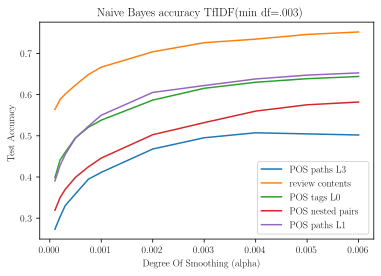
\includegraphics[width=8cm]{figures/nb_x_alpha.pdf}
         \caption{Holding document frequency constant, we vary the $\alpha$ parameter and measure the response of accuracy for Multinomial Naive Bayes.}
         \label{fig:nb_x_alpha}
\end{figure}
We report our results Figure~\ref{fig:clf_acc_x_min_df}. From a minimum document frequency of 0.001, performance of the SVM decreases linearly for review contents (word counts). We take this as an indication that the feature space is sparse, and that the descriptive value of all word term frequencies is roughly uniform. Review contents has a higher $y$ intercept and the highest maximum, but the downward slopes of part of speech based features are lower. This seems to indicate that for certain domains where there are very few documents, and where words don't co-occur across documents, part of speech frequencies may be the best available features.

\subsection{Naive Bayes and Smoothing}


We varied the alpha parameter of naive bayes, shown in Figure~\ref{fig:nb_x_alpha}. All features respond well to smoothing on $[0.001, 0.003]$. Beyond that, all features reach a plateau. The poorer performance with more complex features is consistent with our understanding that combinatorially, there are many more possible length 2 paths than length 1 paths, meaning the feature space is much sparser. With 100 authors at 50 documents each, it is far too sparse to train naive bayes well, when holding minimum document frequency constant. It is possible that an unexplored part of this feature space works better for naive bayes.

The word content in reviews and nested pairs behave similarly, plateauing after a substantial increase. But longer paths drop off in accuracy after the increase. This seems to indicate that many useful features were dropped because the minimum document frequency was too low. The longer the paths are, the more sparse the features get. It is likely that a greater number of sentences per document would result in less sparsity.


\subsection{Features Working Together}

Up to this point, all of the features we have run through the model were used in isolation. We hypothesized using a combination of features can enhance performance. After concatenating all features up to and including L1 bigrams, our SVC topped out at 0.829 accuracy compared to 0.94 with all other factors held constant. We suspect that since some of our features are much denser than word counts (POS tags L0) and some are much sparser (POS paths L1), we are drowning out the descriptive word counts with competing information. Standardizing each individual feature before concatenation is one possible route to fixing this. More work in feature selection is needed to discern how word counts and path features can be made to cooperate in this context.

\subsection{Previously Seen Documents}

We wanted to know how sensitive our system was to the prior number of training examples. We tested this by varying the percent of our total data used for testing and training and we report results in Figure~\ref{fig:prev_seen}. When trained with 18 documents and asked to predict the remaining two, we reach the highest accuracy of 0.94 in the support vector classifier and 0.81 in the naive bayes classifier.

\subsection{Greater Number of Authors}

When expanded to 500 authors with 50 documents each, the accuracy of our models suffered greatly compared to the 100 authors. As we gave less thought to review length of the reviews compared to the 100 author dataset (where we chose the longest reviews of each author), we ended up with less than .5 accuracy at best. More work is needed to expand and improve our models.

\section{Conclusion}

\subsection{Applications}

Since this is a generic stylometric feature extraction tool, it can be applied even beyond the author attribution problem. Path features followed by the TF-IDF vectorizer is essentially a method for vectorizing sentence structure. Wherever sentence complexity could prove to be an informative feature, generalized part of speech paths may be used as an additional set of features to enhance performance of existing feature sets. 

\subsection{Future Work}

In terms of novelty, using token-independent path-based features is not new for source code authorship attribution, but it is quite novel for English. We wonder if this technique can be applied to other languages as well. More experimentation is also needed to flesh out different parameters such as the number of authors, document length, topics, and so on. As mentioned previously, the results are promising and if our work is expanded upon, it might prove to be a valid additional technique for English authorship attribution. 

\section*{Acknowledgements}

We acknowledge Isaac Lapides for his valuable contributions in the planning stages of our project. We thank \citeauthor{Kitaev-2018-SelfAttentive} for their work on the Berkeley Neural Parser that made this work possible. Finally, we thank \citeauthor{klaus_greff-proc-scipy-2017} for the Python Sacred framework which facilitates rapid iteration in experimentation and encourages reproducible research.
%------------------------------------------------
\bibliography{acl2020}
\bibliographystyle{acl_natbib}

\section*{Contributions}

Anthony was our data specialist, ingesting and preprocessing the raw data into a usable form for downstream classifiers and working through many edge cases until we had our operative dataset. Blake led the experiment automation and charting of the outputs. Blake also wrote the parse tree extraction and path feature extraction scripts. We worked together on the experimentation and collaborated on hyperparameter tuning.

Blake was the overall leader with paper writing, migrating our working drafts into the appropriate \LaTeX{} template. Anthony wrote about our dataset creation, populated results and analyses for the 500 author dataset, and wrote future work. 

\end{document}
